\newpage
\exer{4}


\textbf{\underline{ex4.html}}
\vspace{0.1cm}

\lstinputlisting[style=htmlstyle]{Code/EX4/ex4.html}

\vspace{1.5cm}

\textbf{\underline{Output}}

\vspace{0.1cm}
\begin{center}
\setlength{\fboxrule}{2pt} % Set border thickness
\fbox{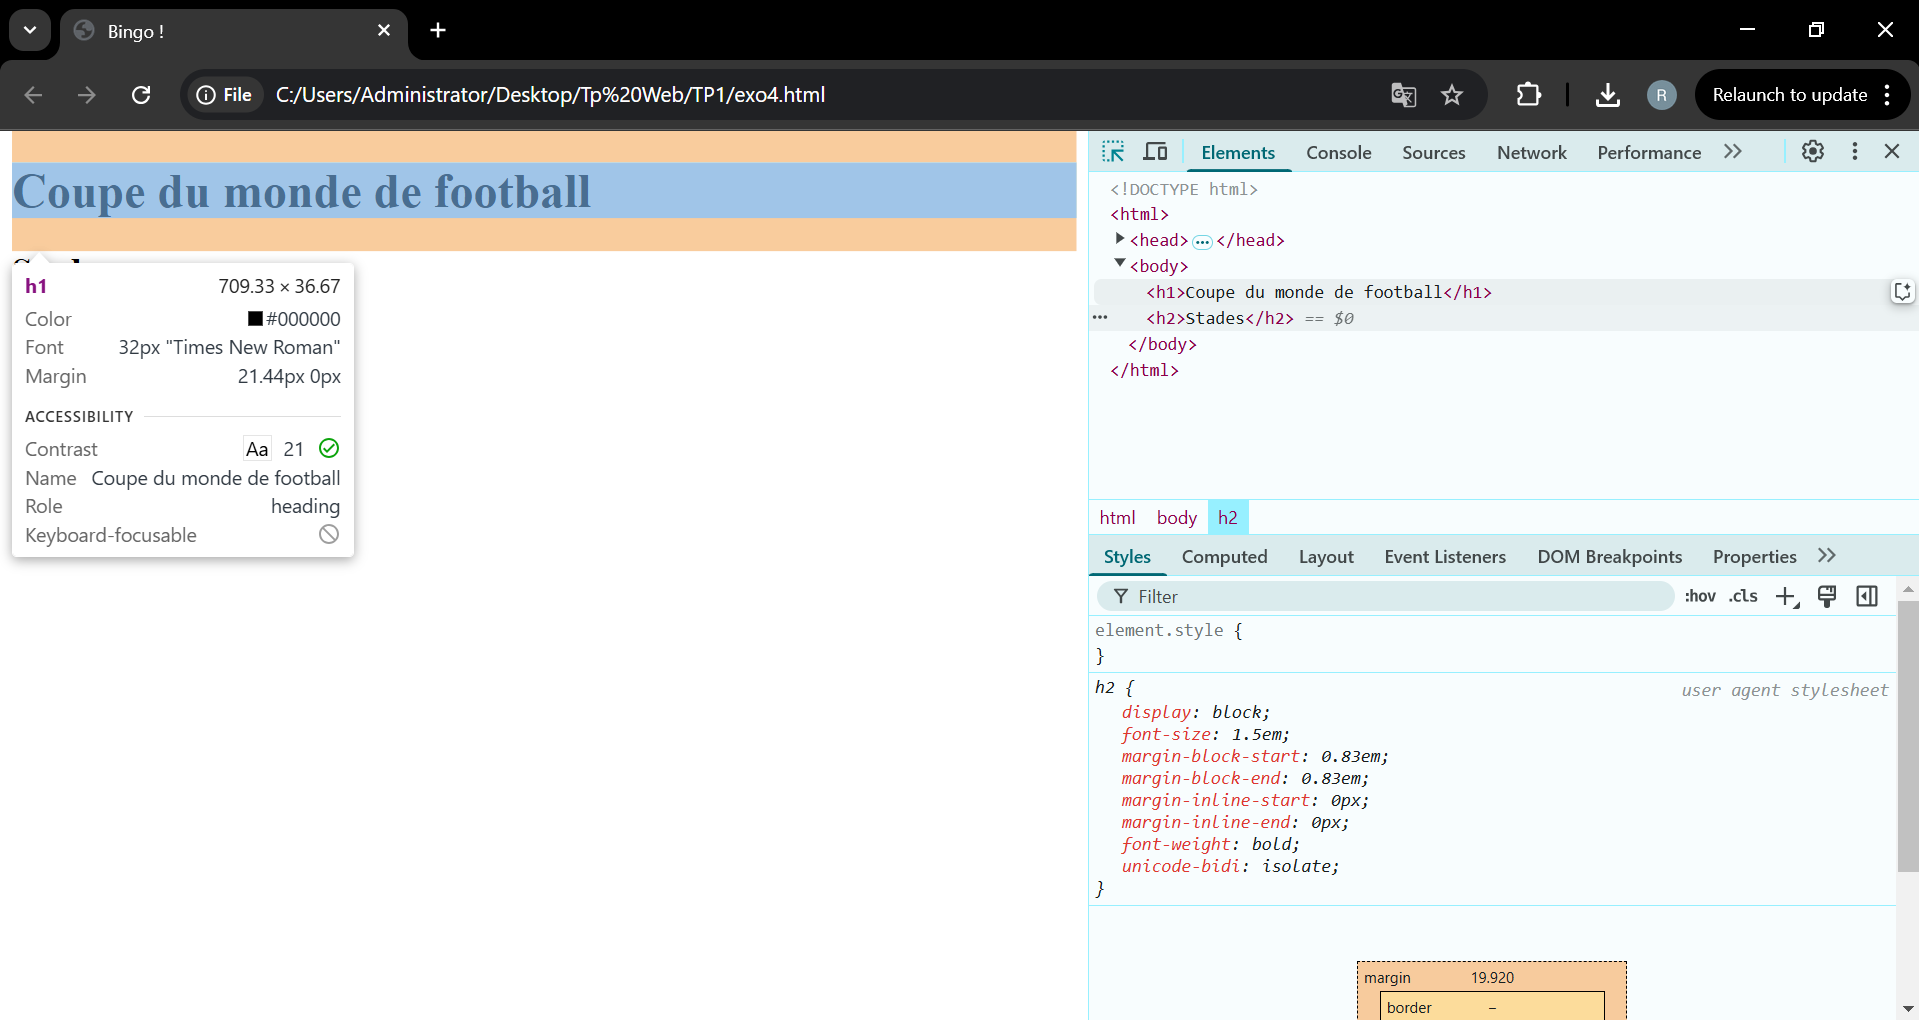
\includegraphics[height=0.4\textheight]{Code/EX4/ex4.1.PNG}}
\end{center}

\begin{center}
\setlength{\fboxrule}{2pt} % Set border thickness
\fbox{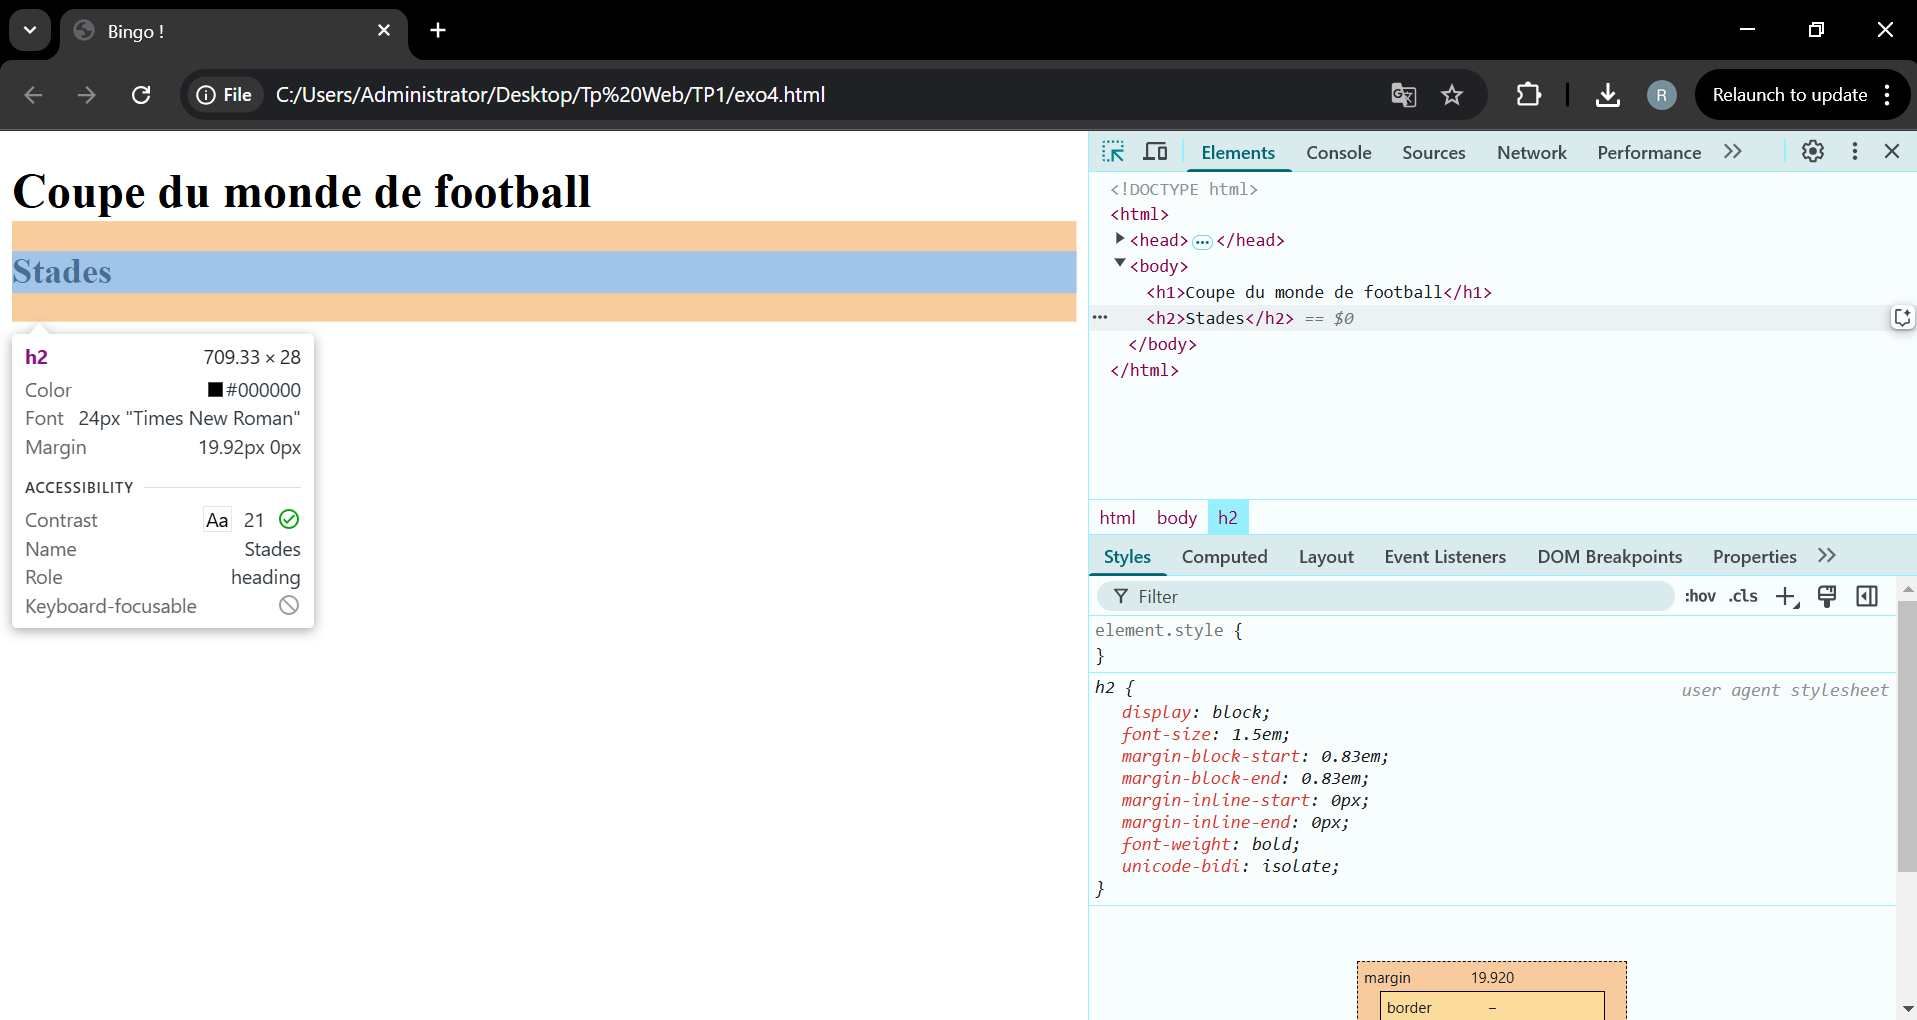
\includegraphics[height=0.4\textheight]{Code/EX4/ex4.2.PNG}}
\end{center}



\vspace{1cm}

\begin{prettyBox}{Observation}{myblue}
    \begin{itemize}
        \item \(<\)h1\(>\) et \(<\)h2\(>\) sont des elements block.
    \end{itemize}
\end{prettyBox}
